<<<<<<< HEAD
%!TEX root = ../main.tex
\section{Windows}

\subsection{Install Python}

\subsubsection{Obtain the Python binary}

First, download a Python installer from the official Website, which can be found at \url{https://www.python.org/download/}. Be sure to select an installer, not source packages. It should not matter which version you use, but recommended is the either the newest version of 2.7 or the newest version of 3.X. It is a matter of taste, and might depend on which version you might already have installed. But setlx2py should run with all newer versions of standard Python.

The setup itself is self-explanatory, just run the executable as usual. When you decide where to install, it is recommended to let Python install where it wants. If you choose a different installation path, remember where it was, you will need that information in the next step. The location of the Python installation is called \texttt{\$PYHOME} for further reference.

\subsubsection{Setting the \$PATH}

Now you could run Python with the command

\begin{lstlisting}{breaklines=true, language=bash}
$ $PYHOME\python.exe
\end{lstlisting}

Typing the full path is very tedious. To ease the usage of the Python interpreter, Windows has the feature of the \texttt{\$PATH}-Variable. Whenever you insert a command without a fully specified path, it looks in the folders you specified in that variable, and looks for a match. There are two ways to add a program to the path variable. Open a Powershell with either \keys{Win + R + `powershell' + Enter}. Insert the follwing command in the just opened window: 

\begin{lstlisting}{breaklines=true, language=bash}
$ [Environment]::SetEnvironmentVariable("Path", "$env:Path;C:\Python27\;C:\Python27\Scripts\", "User")
\end{lstlisting}

In that example, we used Python 2.7. If you installed another version of python, or used a different \texttt{\$PYHOME}, adjust the part of \textit{C:\textbackslash Python27} to reflect the differences. 

Close the shell and open it again. You should now be able to open a Python prompt with entering

\begin{lstlisting}{breaklines=true, language=bash}
$ python
\end{lstlisting}

in the shell. 

\begin{figure}[ht]
    \centering
    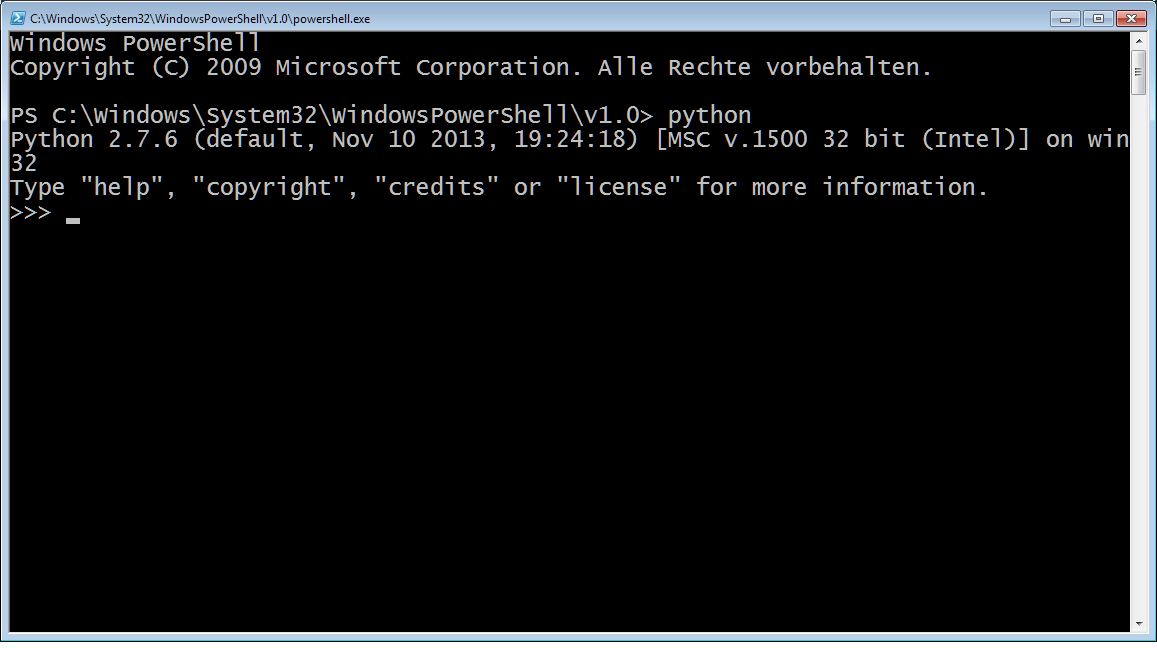
\includegraphics[width=0.8\textwidth]{img/install-python.png}
    \caption{Running python from a shell without fully specified path}
    \label{fig:install-python}
\end{figure}

\subsection{Install package manager}

Python allows installing packages in a very easy way. Sadly, it does not ship with a package manager. Therefore, it is installed in the next step. Download

\url{https://raw.github.com/pypa/pip/master/contrib/get-pip.py}

Open a shell and change the directory to the folder to where you downloaded it (the \keys{cd + \$FOLDERNAME} command does that for you). Now run 

\begin{lstlisting}{breaklines=true, language=bash}
$ python \.get-pip.py
\end{lstlisting}

You should see a confirmation that it is installed everything successfully like in Fig. \ref{fig:install-pip}.

\begin{figure}[ht]
    \centering
    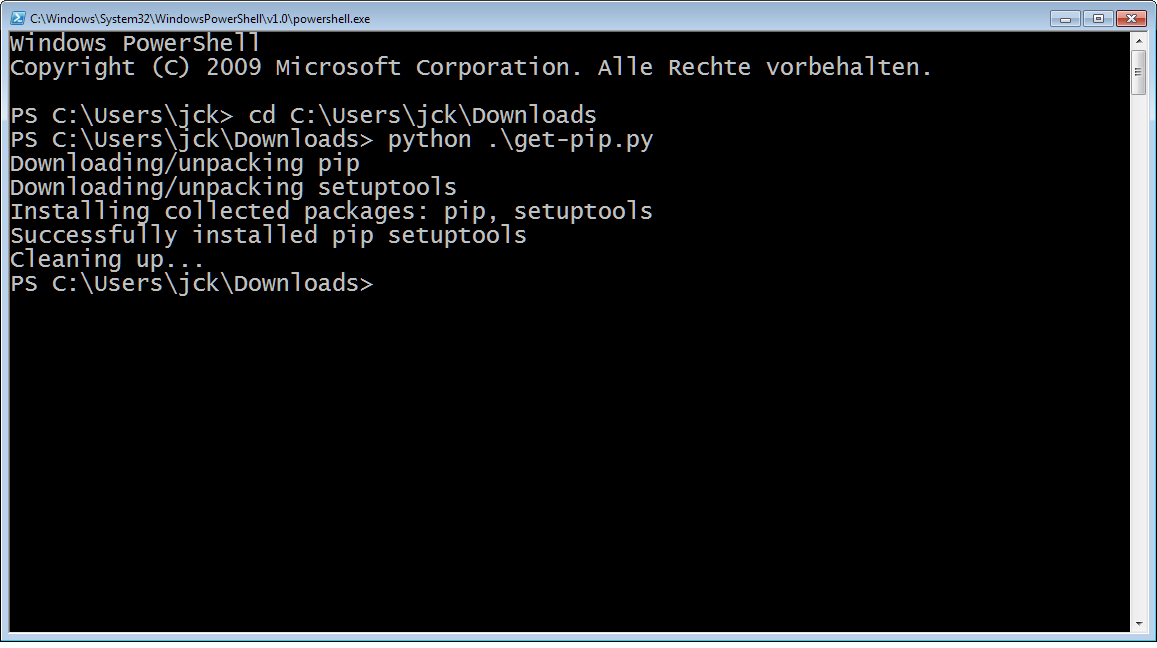
\includegraphics[width=0.8\textwidth]{img/install-pip.png}    
    \caption{Installing the package manager pip}
    \label{fig:install-pip}    
\end{figure}

\subsection{Install binary dependencies}

Setlx2py uses internally some platform-specific binary libraries. It is possible to compile these for Windows with some effort, but they can be found precompiled already. 

Download the fitting version of the \texttt{blist} package (for the curious, it offers better/more advanced data structures) and install it. Be sure to download the same architecture as you did for Python (32- or 64-bit), else you get an error with a name of `Cannot install' or similar. The package itself can be obtained from

\url{http://www.lfd.uci.edu/~gohlke/pythonlibs/#blist}

\subsection{Install Python dependencies}

Download the setlx2py archive from 

\url{https://github.com/Rentier/setlx2py/archive/master.zip}

and extract it. Open a shell and change the working directory to the folder where the \texttt{REQUIREMENTS.txt} file can be found. With the power of \texttt{pip}, all other dependencies can now be installed with 

\begin{lstlisting}{breaklines=true, language=bash}
$ pip install -r REQUIREMENTS.txt
\end{lstlisting}

The package manager now retrieves all the dependencies specified in the given file. After some time, it messages `Successfully installed'. Everything is now in place to actually use setlx2py.

\begin{figure}[ht]
    \centering
    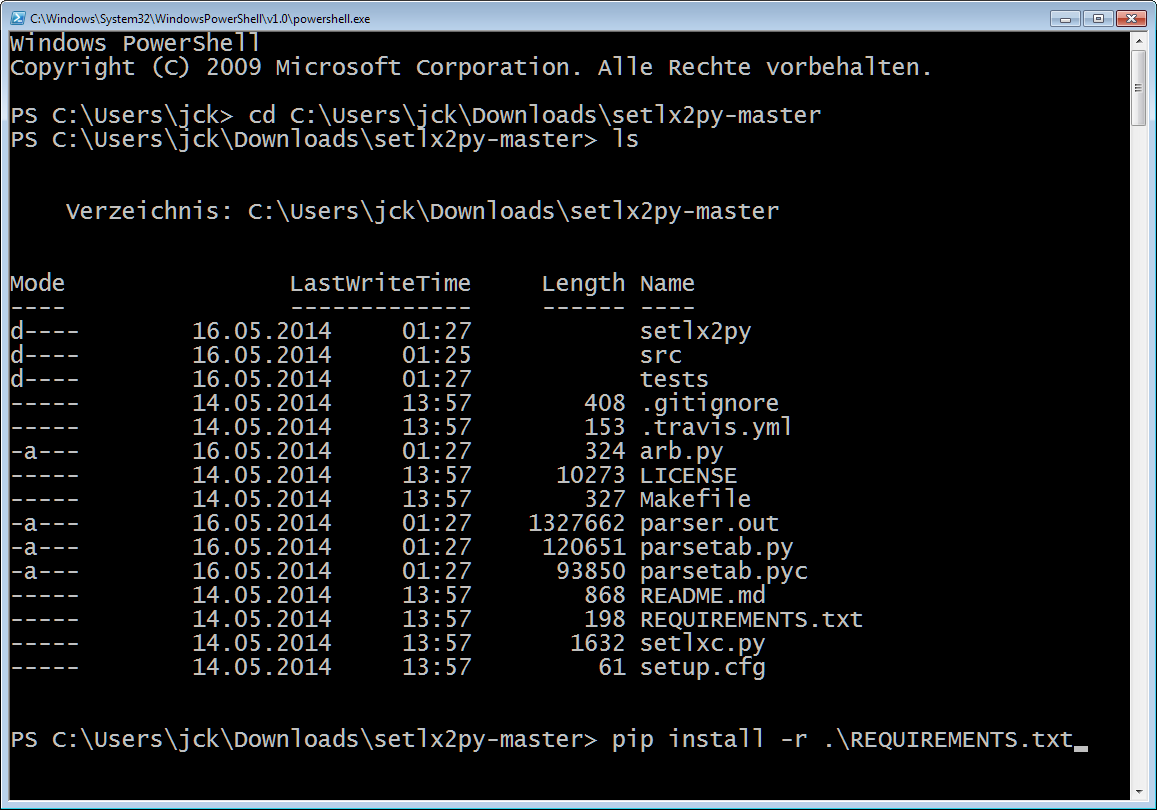
\includegraphics[width=0.8\textwidth]{img/install-reqs.png}
    \caption{Installing the dependencies of setlx2py with pip}
    \label{fig:install-req}
\end{figure}
=======
%!TEX root = ../main.tex
\section{Windows}

\subsection{Install Python}

\subsubsection{Obtain the Python binary}

First, download a Python installer from the official Website, which can be found at \url{https://www.python.org/download/}. Be sure to select an installer, not source packages. It should not matter which version you use, but recommended is the either the newest version of 2.7 or the newest version of 3.X. It is a matter of taste, and might depend on which version you might already have installed. But setlx2py should run with all newer versions of standard Python.

The setup itself is self-explanatory, just run the executable as usual. When you decide where to install, it is recommended to let Python install where it wants. If you choose a different installation path, remember where it was, you will need that information in the next step. The location of the Python installation is called \texttt{\$PYHOME} for further reference.

\subsubsection{Setting the \$PATH}

Now you could run Python with the command

\begin{lstlisting}{breaklines=true, language=bash}
# $PYHOME\python.exe
\end{lstlisting}

Typing the full path is very tedious. To ease the usage of the Python interpreter, Windows has the feature of the \texttt{\$PATH}-Variable. Whenever you insert a command without a fully specified path, it looks in the folders you specified in that variable, and looks for a match. There are two ways to add a program to the path variable. Open a Powershell with either \keys{Win + R + `powershell' + Enter}. Insert the follwing command in the just opened window: 

\begin{lstlisting}{breaklines=true, language=bash}
# [Environment]::SetEnvironmentVariable("Path", "$env:Path;C:\Python27\;C:\Python27\Scripts\", "User")
\end{lstlisting}

In that example, we used Python 2.7. If you installed another version of python, or used a different \texttt{\$PYHOME}, adjust the part of \textit{C:\textbackslash Python27} to reflect the differences. 

Close the shell and open it again. You should now be able to open a Python prompt with entering

\begin{lstlisting}{breaklines=true, language=bash}
# python
\end{lstlisting}

in the shell. 

\begin{figure}[ht]
    \centering
    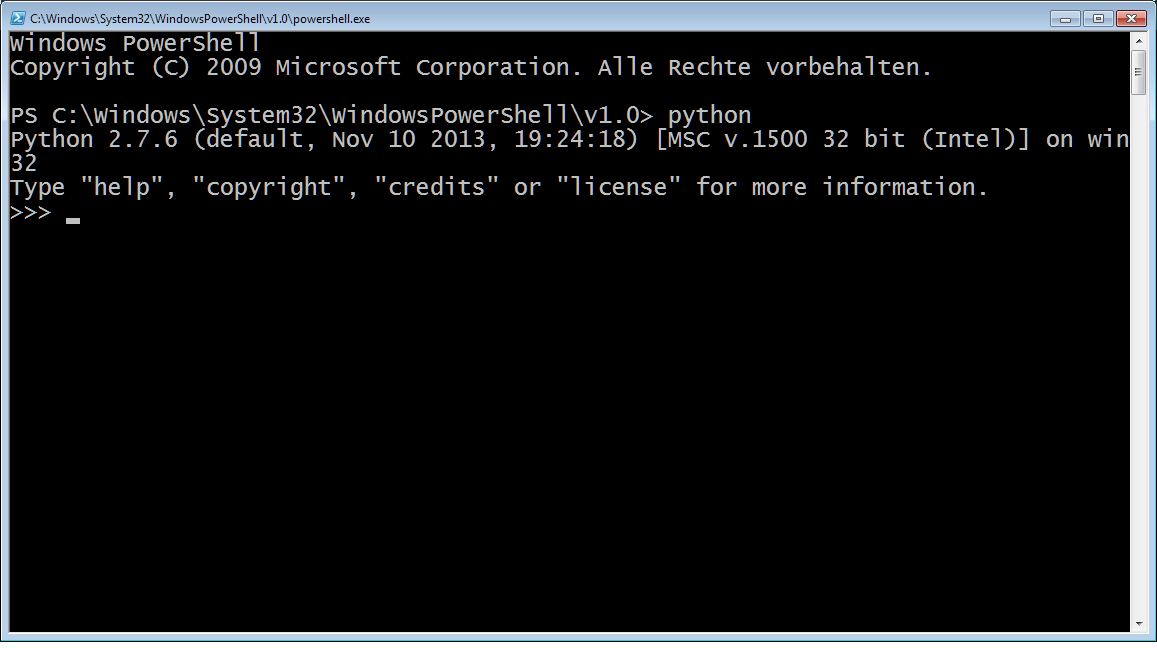
\includegraphics[width=0.8\textwidth]{img/install-python.png}
    \caption{Running python from a shell without fully specified path}
    \label{fig:install-python}
\end{figure}

\subsection{Install package manager}

Python allows installing packages in a very easy way. Sadly, it does not ship with a package manager. Therefore, it is installed in the next step. Download

\url{https://raw.github.com/pypa/pip/master/contrib/get-pip.py}

Open a shell and change the directory to the folder to where you downloaded it (the \keys{cd + \$FOLDERNAME} command does that for you). Now run 

\begin{lstlisting}{breaklines=true, language=bash}
# python \.get-pip.py
\end{lstlisting}

You should see a confirmation that it is installed everything successfully like in Fig. \ref{fig:install-pip}.

\begin{figure}[ht]
    \centering
    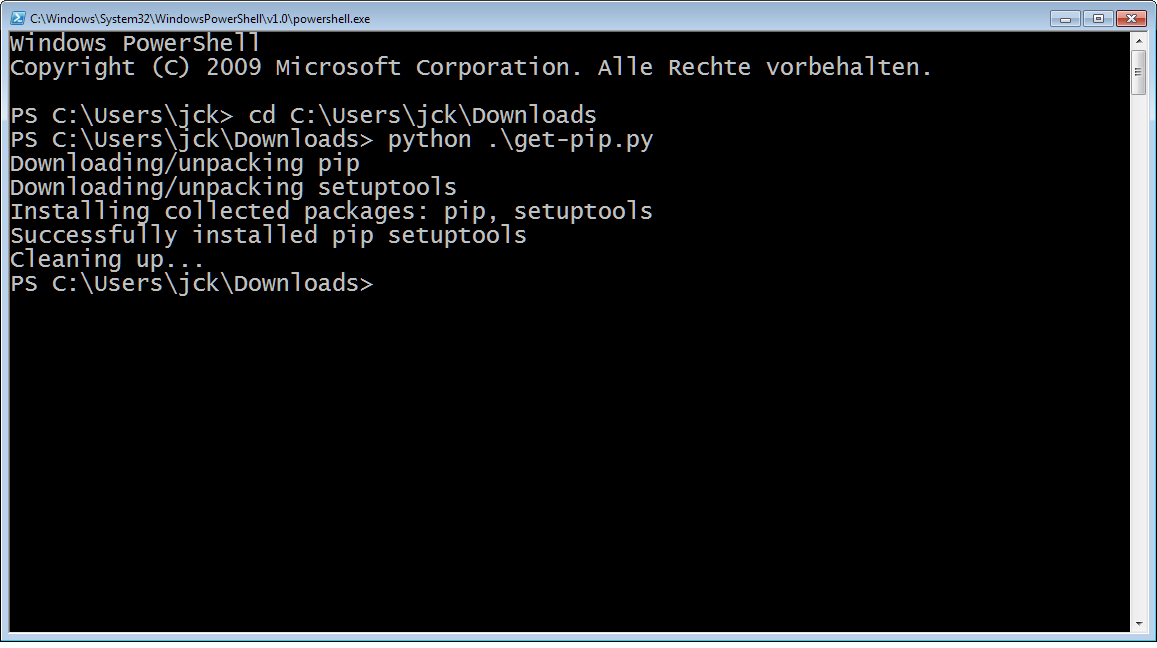
\includegraphics[width=0.8\textwidth]{img/install-pip.png}    
    \caption{Installing the package manager pip}
    \label{fig:install-pip}    
\end{figure}

\subsection{Install binary dependencies}

Setlx2py uses internally some platform-specific binary libraries. It is possible to compile these for Windows with some effort, but people offer them precompiled already. Download the fitting version of the \texttt{blist} package (for the curious, it offers better/more advanced data structures) and install it. Be sure to download the same architecture as you did for Python (32- or 64-bit), else you get an error with a name of `Cannot install' or similar. The package itself can be obtained from

\url{http://www.lfd.uci.edu/~gohlke/pythonlibs/#blist}

\subsection{Install dependencies}

Download the setlx2py archive from 

\url{https://github.com/Rentier/setlx2py/archive/master.zip}

and extract it. Open a shell and change the working directory to the folder where the \texttt{REQUIREMENTS.txt} file can be found. With the power of \texttt{pip}, all other dependencies can now be installed with 

\begin{lstlisting}{breaklines=true, language=bash}
# pip install -r REQUIREMENTS.txt
\end{lstlisting}

The package manager now retrieves all the dependencies specified in the given file. After some time, it messages `Successfully installed'. Everything is now in place to actually use setlx2py.

\begin{figure}[ht]
    \centering
    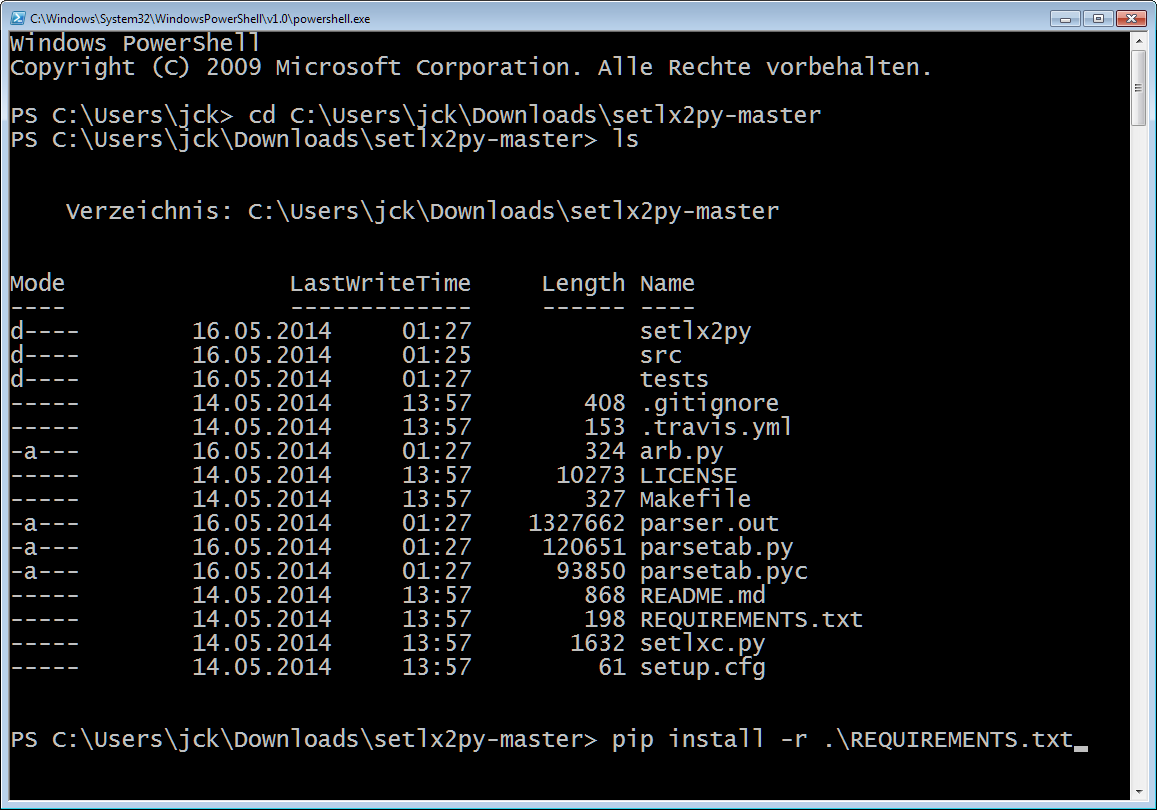
\includegraphics[width=0.8\textwidth]{img/install-reqs.png}
    \caption{Installing the dependencies of setlx2py with pip}
    \label{fig:install-req}
\end{figure}

\subsection{Use setlx2py}

Now that all prequisites are installed, the actual compiler can be downloaded. This step uses the previously installed package manager, so it only requires one command to install setlx2py. Grab an open shell, and issue the following command:

\begin{lstlisting}{breaklines=true, language=bash}
# pip install git+git://github.com/Rentier/setlx2py.git@master
\end{lstlisting}
>>>>>>> 6640584894f5245d515ca7633dadcb0b4d99f7b3
